\begin{abstract}
The study of Earth atmosphere and its dynamic is a very interesting topic for
weather accurate forecasting. Even nowadays, with improved numerical methods
and complex atmospheric models, we are not able to determine an accurate weather
prediction if the conditions are extremes or the prediction times increases.\\

The purpose of the \textbf{A}tmospheric \textbf{D}ynamics \textbf{M}ission Aeolus
is to further develop the knowledge of Earth atmosphere and weather models by
studying the winds speed and direction around the Earth.
In this study is going to be analysed why the instrument developed for this
mission is the better solution for this purpose.\\

ADM-Aeolus is an Earth Observation satellite manufactured by Airbus Defence and Space
and operated by the European Space Agency (ESA), that as launched on August 22, 2018
from the Guiana Space Centre, in Kourou (French Guiana).\\
\end{abstract}

\section{Introduction}

The atmosphere is a very complex system which is governed by fluids equations,
which solutions tends to be chaotic and the simulations to predict its evolution
are not able to give precise forecasts for several days or weeks. It's known
that exists some steady great scale flows arounf the Earth, due to solar irradiation
and Coriolis effect. This currents are shown in figure \ref{fig:earth_winds}\\

\begin{figure}[h]
	\centering
	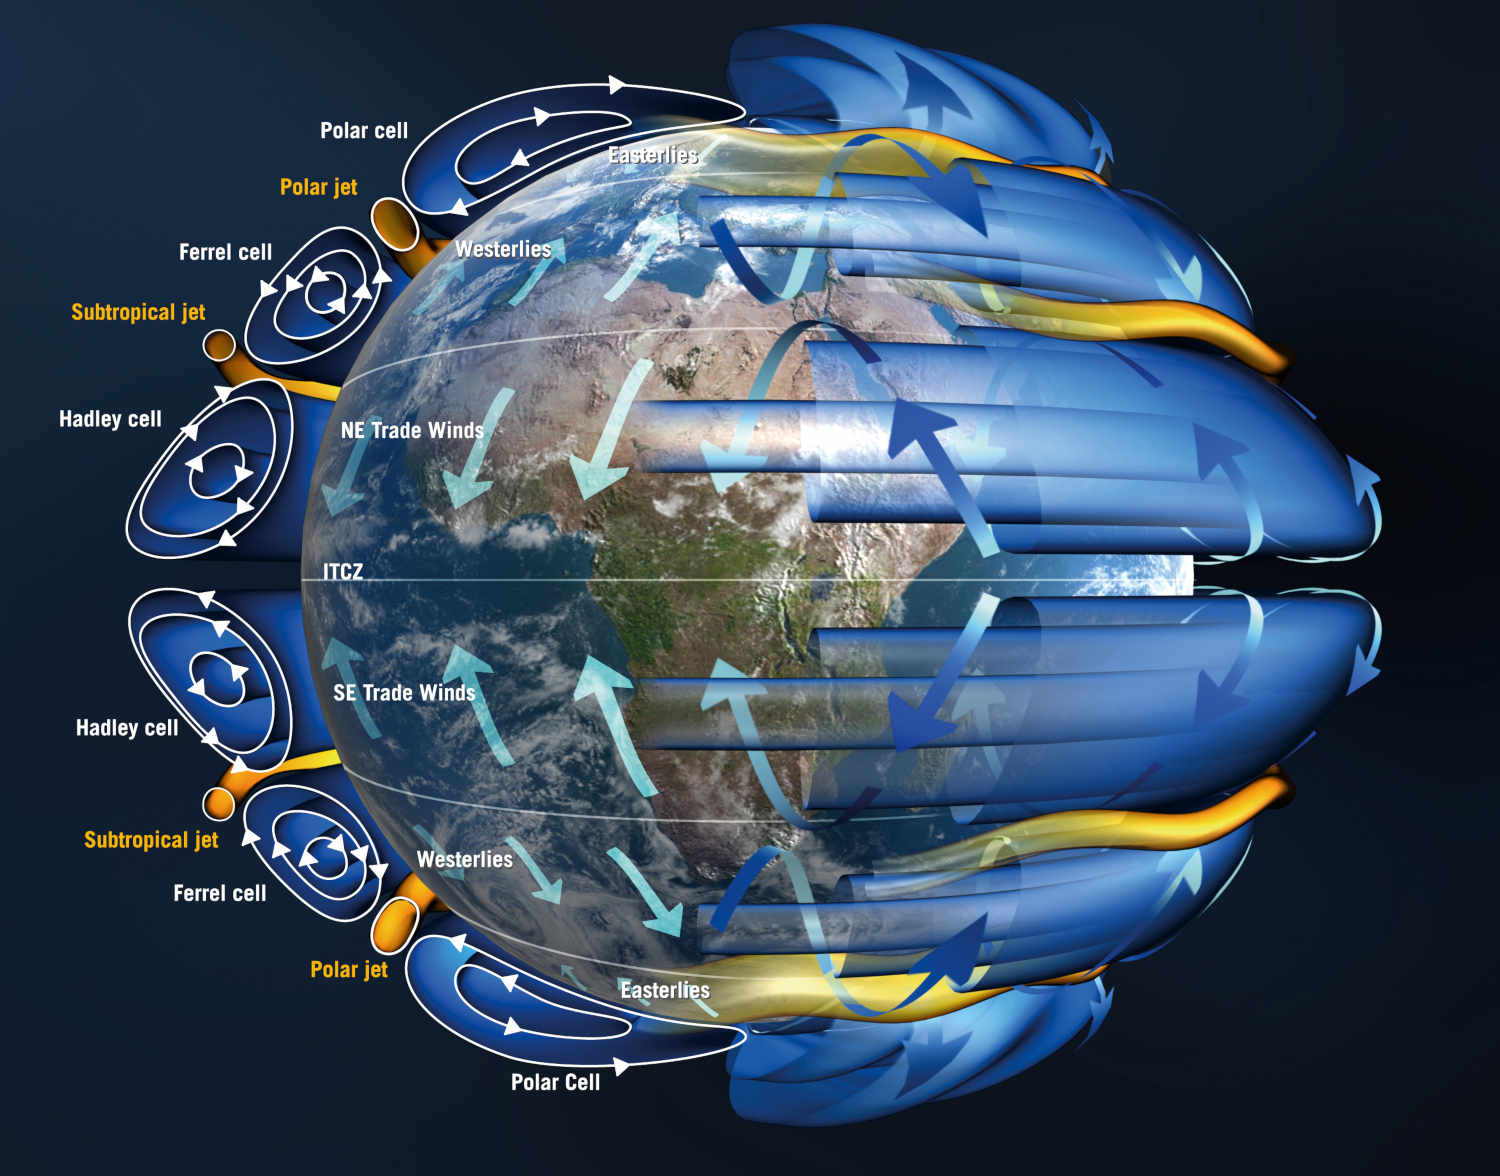
\includegraphics[width=0.8\textwidth]{img/Earth_winds.jpg}
	\caption[Earth winds circulation]{A model of Earth's atmosphere air circulation, transporting heat
	from equatorial regions to poles and returning cooled air to the tropics.
	The circulation in each hemisphere consists of three cells, creating two
	important jets in each hemisphere. Credits: ESA/AOES Medialab \cite{earth_winds}}
	\label{fig:earth_winds}
\end{figure}


Something that would help improving the weather predictions is to better know
the winds profile in every layer of the atmosphere, globally, and with much better
time resolution. This study has been performed in the past by using flying probes
as high altitude balloons, or other unmanned flying devices which were able to
measure the winds speed but in a local area, not in every moment, nor every altitude.\\

The mission ADM-Aeolus is intended to provide this global observations of winds,
for every altitude in the atmosphere and with a resolution that will satisfy the
requirements of the World Meteorological Organization (WMO). ADM-Aeolus will
be the first satellite to directly observe the Earth’s wind profiles from space.
\cite{Endemann2004}\\

The Mission was launched this year on 22 of August onboard of a Vega rocket, manufactured
by the Italian company Avio, from the Guiana Space Centre, one of the usual launch
facilities of the European Space Agency located in Kourou, French Guiana. The total
mass of the satellite is 1360kg, which includes 266kg of fuel, and it is orbiting
Earth in a 320km height sun-synchronous orbit, with an inclination of 96.7º and a period
of 90.7 minutes \cite{aeolus_n2yo.com}, with an estimated lifetime of at least
3 years, due to his relative low orbit altitude.

\section{Payload: ALADIN}

To accomplish the mission objective of studying the winds in Earth atmosphere, the
selected payload is called ALADIN, which stands for \textbf{A}tmospheric \textbf{LA}ser
\textbf{D}oppler \textbf{IN}strument. This instrument is able to measure the
wind speed and direction in every layer of the atmosphere covering all the Earth.\\

The way in this instrument works is by pointing a UV-LASER beam into the atmosphere
and observing the back-scattered light from it, which would suffer Doppler-effect
due to the velocity of air molecules moving withing the atmospheric currents, as
is depicted in figure \ref{fig:scanning}, employing the DWL (Doppler Wind Lidar) measuremnent
technique, along the LOS (Line-of-Sight).\\

\begin{figure}[h]
	\centering
	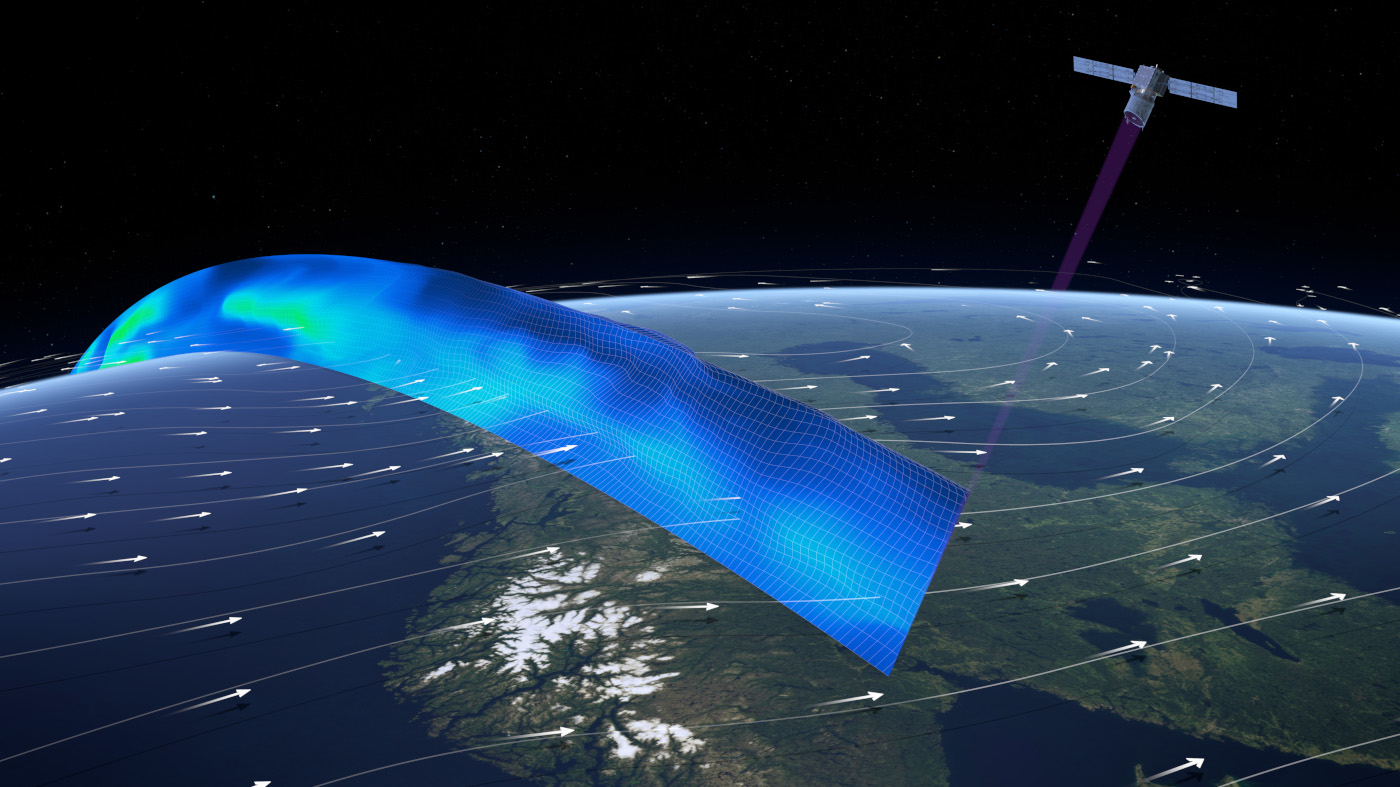
\includegraphics[width=0.9\textwidth]{img/Winds_profile.jpg}
	\caption[Wind profile scanning]{Artistic impression of Aeolus scanning Earth winds profiles.
	Credits: ESA/ATG medialab \cite{scanning}}
	\label{fig:scanning}
\end{figure}

By sending a pulsed high power UV laser bean into the atmosphere it can be analysed
the Rayleigh scattered light coming from it with a delay which accounts for the
distance where the light was dispersed and and frequency shift related with the velocity
of the air. Computing that signal it can be obtained the wind profile in the scanned
LOS. (Figure \ref{fig:lidar})\\

\begin{figure}[h]
	\centering
	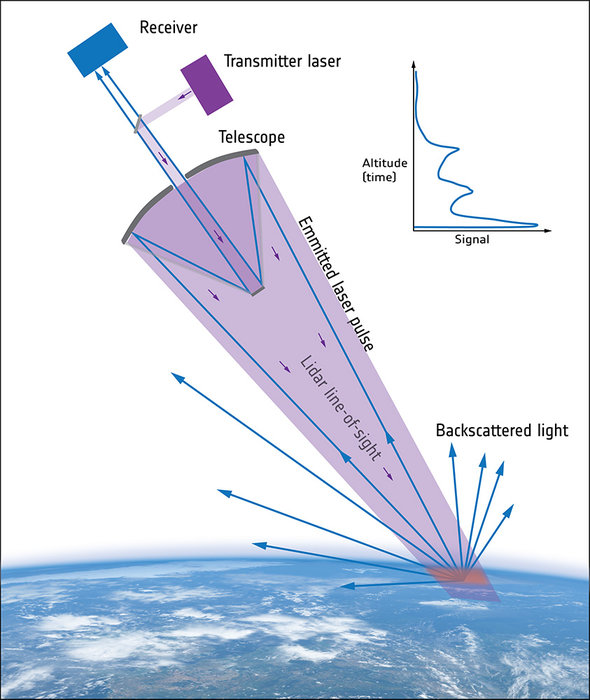
\includegraphics[width=0.7\textwidth]{img/20170519_Lidar_concept_ESA.jpg}
	\caption[Doppler Wind Lidar measurement technique]{Aladin
	instrument incorporates two powerful lasers, a large telescope and very
	sensitive receivers. The laser generates ultraviolet light that is beamed
	towards Earth. This light bounces off air molecules and small particles
	such as dust, ice and droplets of water in the atmosphere. The fraction
	of light that is scattered back towards the satellite is collected by
	Aladin’s telescope and measured. Credits: ESA \cite{lidar_concept}}
	\label{fig:lidar}
\end{figure}

The satellite is placed in a polar synchronous orbit, with a mean altitude of
320km (perigee: 314.5km, apogee: 321.4km), with an inclination of 96.97º. \ref{aeolus_n2yo.com}
The local equator crossing for the ascending node is at 18h and at 6h for the descending
node, which is called dawn-dusk orbit, because the satellite is always flying over
the sunrise or sunset line. This allows the satellite have a continue illumination from
the Sun, allowing the solar panels to be continuously generating power. It's also
important because, in the case of Aeolus, the Laser could be pointing always to the
night part with a constant angle, as we can see in the figure \ref{fig:geometry}.\\

\begin{figure}[h]
	\centering
	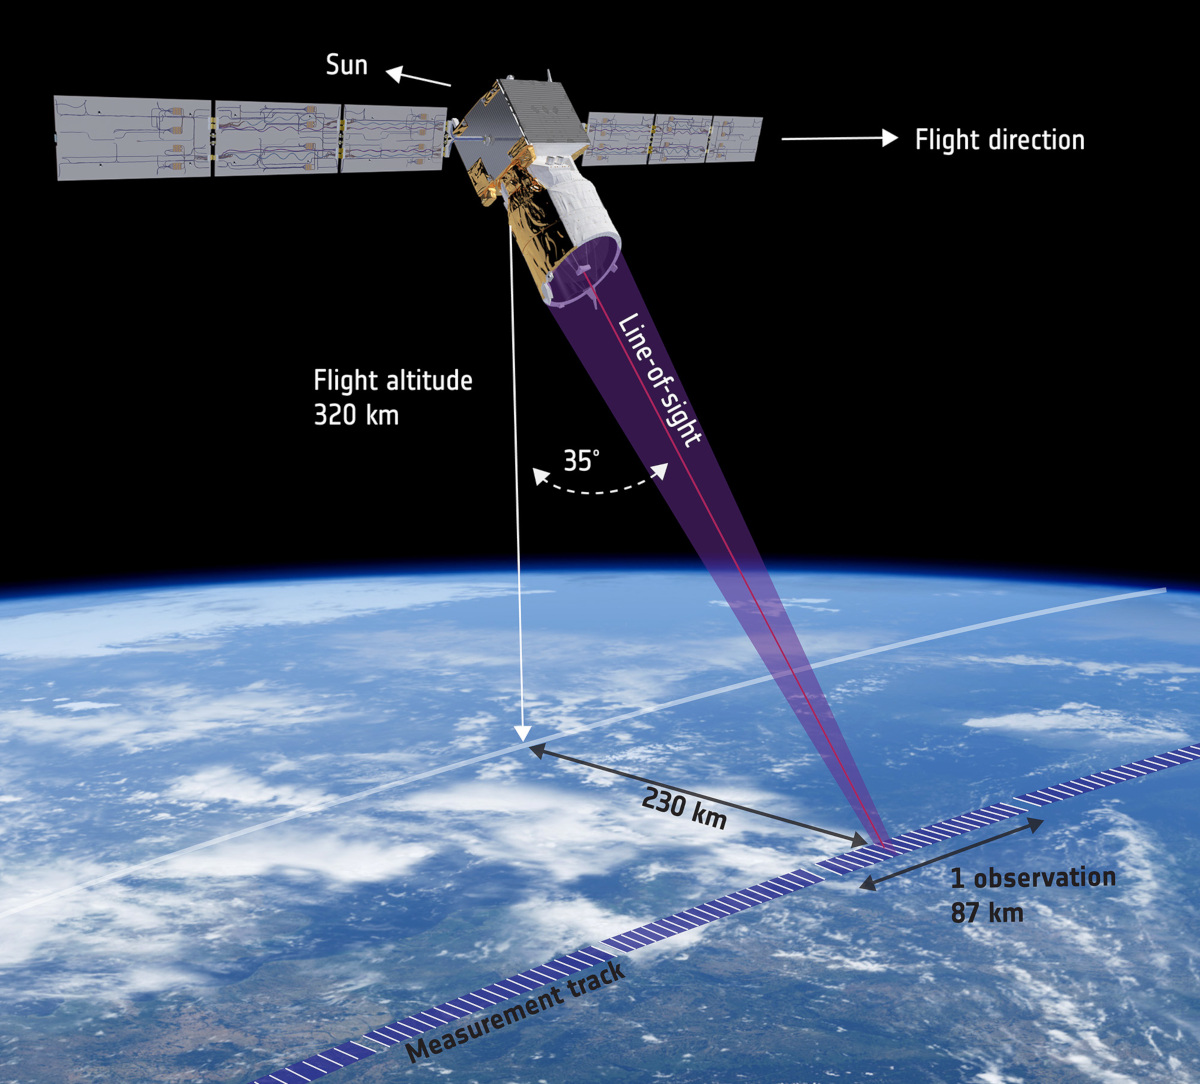
\includegraphics[width=0.7\textwidth]{img/geometry.jpg}
	\caption[Geometry of measurements]{The LOS is pointing 35° off nadir,
	away from the Sun, to the dark side. Credits: ESA/ESTEC \cite{geometry}}
	\label{fig:geometry}
\end{figure}

The orbit period is 90.7 minutes, and it has a revisit time of 7 days, (111 orbits),
after that period, the orbits repeat the same ground track. So the global wind data
will update every 7 days globally.\\

The payload itself is composed by many systems and devices. The overall ALADIN
instrument architecture is based on a 60 mJ diode-pumped frequency-tripled
Nd:YAG (Neodymium-doped Yttrium Aluminium Garnet) laser operating in the
ultraviolet spectrum. The instrument consists of three main parts: the transmitter,
a combined Mie and Rayleigh backscattering receiver device, and the opto-mechanical
subsystem, which mainly consists in a 1.5 m diameter telescope.\\

Both Mie and Raileigh scattering refers to the phenomena of light dispersion when
its interacts with spherical bodies, as, for example, small water droplets, aerosol
or dusk specks present in the atmosphere. A picture of the complete ALADIN instrument
is shown in figure \ref{fig:full_payload}.\\

\begin{figure}[h]
	\centering
	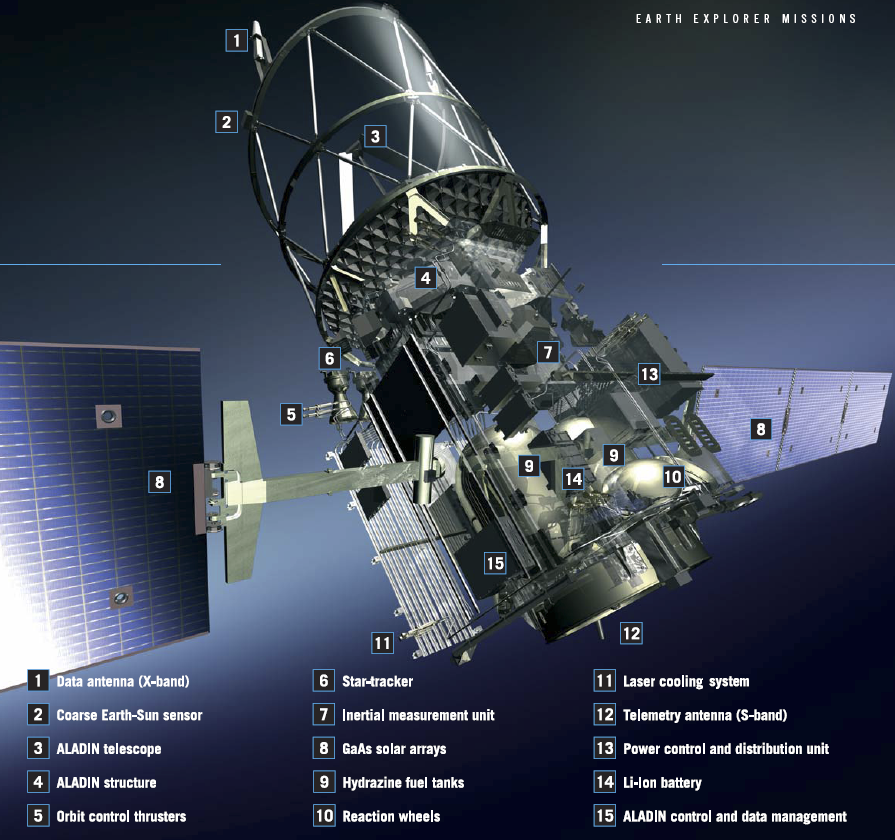
\includegraphics[width=0.8\textwidth]{img/Aeolus_payload_components.png}
	\caption[ALADIN instrument components]{A full picture of Aeolus satellite
	components, indicating also the main ALADIN devices and structures. Credits: ESA \cite{full_payload}}
	\label{fig:full_payload}
\end{figure}

The solar arrays of 13 m span have three panels on each
side. With GaAs cells, they will provide over 2 kW power,
to supply an orbital average power of about 1.4 kW \ref{Endemann2004}.\\

One of the main technological challenges of this mission is related with the
thermal control. The main problem is the large amount of heat generated by the
LASER transmitter, which could affect negatively to the rest of devices like
spectrometers and optics. To deal with this heat, it was implemented a complex
system of heat pipes and a cooling radiator pointing to the shadow side of the
satellite, as shown in figure \ref{fig:radiator}.\\

\begin{figure}[h]
	\centering
	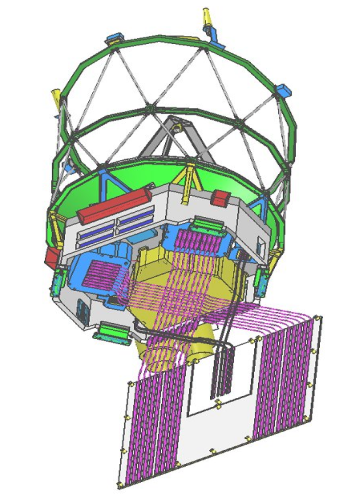
\includegraphics[width=0.6\textwidth]{img/radiator.png}
	\caption[ALADIN thermal control]{The $2m^2$ heat radiator pointing the
	dark side of the satellite, conected with many heat pipes to the LASER
	transmitter. \cite{Endemann2004}}
	\label{fig:full_payload}
\end{figure}

In the figure \ref{fig:optics}, is shown the optical system including the power
laser generators (PLH 1 \& 2), and the Mia/Rayleigh spectrometers. And in the figure
\ref{fig:PLH} the optical bench used for the Power Laser Head is depicted.\\

\begin{figure}[h]
	\centering
	\begin{subfigure}{0.45\textwidth}
		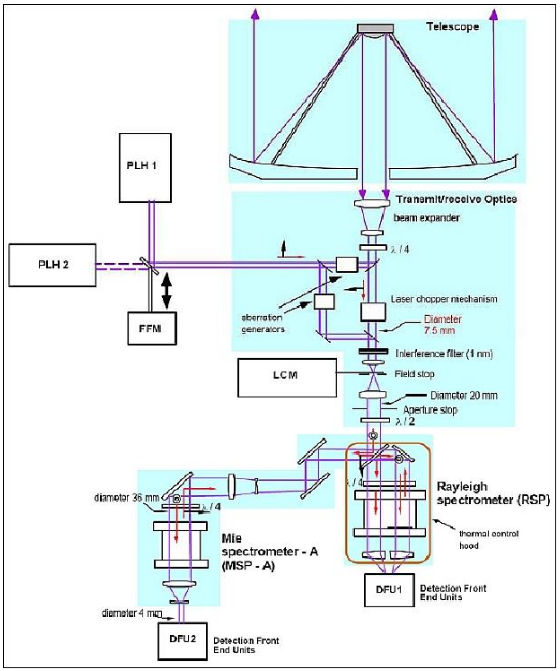
\includegraphics[width=\textwidth]{img/optics.png}
		\caption{ALADIN receiver optics with Rayleigh \& Mie spectrometers. Credits: ESA}
		\label{fig:optics}
	\end{subfigure}
	~
	\begin{subfigure}{0.45\textwidth}
		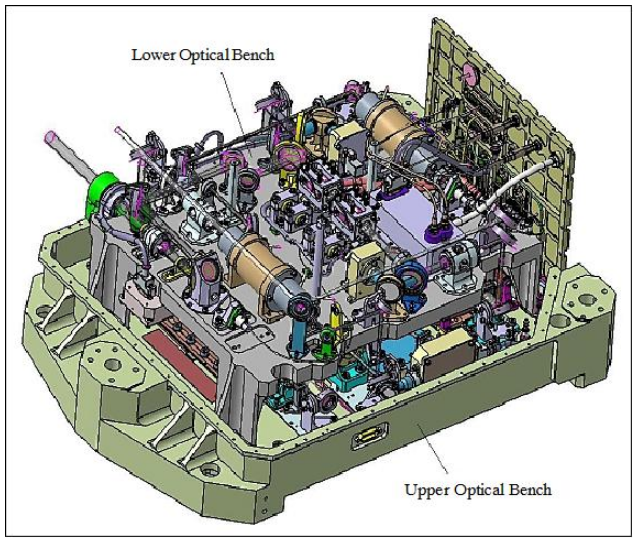
\includegraphics[width=\textwidth]{img/optical_bench.png}
		\caption{Mechanical structure of PLH (Power Laser Head) of ALADIN.
		Credits: Galileo Avionica, ESA}
		\label{fig:PLH}
	\end{subfigure}
	\caption[Optical instruments]{Optical instruments \cite{aeolus_webpage}}
	\label{fig:optical}
\end{figure}

Just to finish, it's interesting to show an image (figure \ref{fig:results}) of the
first recorded data, which was received on September 12 of 2018, just few week after
the satellite launch in August 22. From the deployment of the satellite and the first
data gathered, the satellite is now doing more tests and calibrations procedures in
order to be fully operable after a period of three months.\\

\begin{figure}[h]
	\centering
	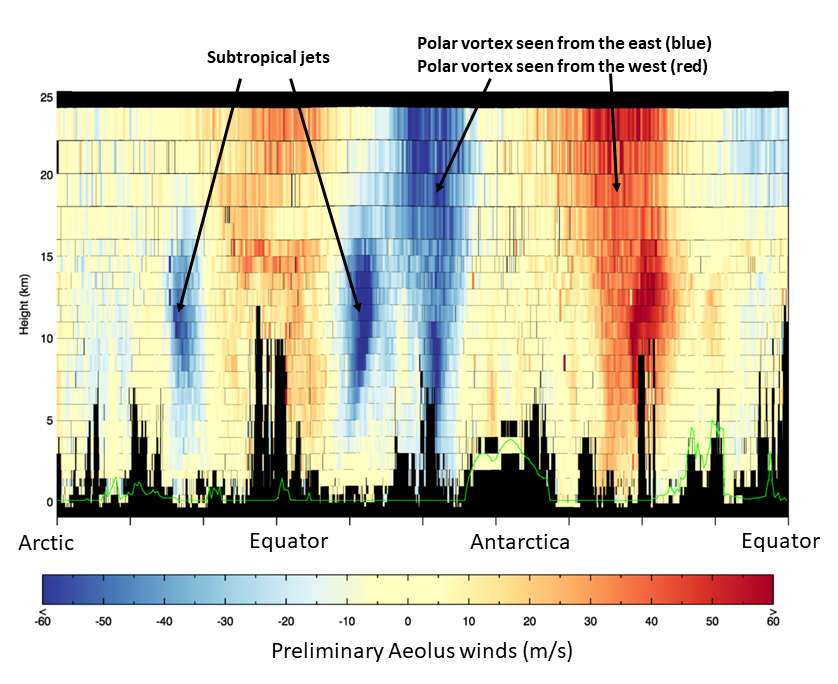
\includegraphics[width=0.9\textwidth]{img/20180912_First_wind_measurement.png}
	\caption[First wind data gathered from Aeolus]{First wind data from ESA’s
	Aeolus satellite. These data are from three quarters of one orbit around
	Earth. The image shows large-scale easterly and westerly winds between
	Earth’s surface and the lower stratosphere, including jet streams. Credits: ESA/ECMWF\cite{first_data}}
	\label{fig:results}
\end{figure}

\clearpage
\section{Conclusions}

As we have seen during the description of the ALADIN payload used in the mission
ADM-Aeolus, the choice of this payload is greatly adequate to perform the mission
objectives of analysing the global winds profiles, because it has proven being able
of recording this data with the accuracy and resolution required.

This is the first time that a Doppler Wind Lidar (DWL) measurement of the Earth
atmosphere is done from the space, and it has been done with an state-of-art instrument
developed during 16 years of high value technological design. As Juan Piñero,
Spacecraft Operations Manager for Aeolus, says:

\begin{center}
\begin{minipage}{0.9\linewidth}
\vspace{5pt}%
{\small
Aeolus’ arrival at the launch site marks the end of 16 years of intensive planning,
testing and construction, by literally generations of engineers and scientists.
}
\end{minipage}
\end{center}
